\documentclass[12pt,a4paper]{article}

\usepackage[utf8]{inputenc}
\usepackage[T5]{fontenc}
\usepackage[vietnamese]{babel}
\usepackage{graphicx}
\usepackage{float}
\usepackage{geometry}
\usepackage{array}
\usepackage{booktabs}
\usepackage{enumitem}
\usepackage{makecell}
\usepackage{amsmath}
\usepackage{amssymb}
\usepackage{hyperref}
\usepackage{tocloft}
\usepackage{titlesec}

\newcommand{\sectionbreak}{\clearpage}
\geometry{top=2cm,bottom=2cm,left=2.5cm,right=2cm}
\hypersetup{
    colorlinks=true,
    linkcolor=black,
    citecolor=black,
    urlcolor=blue
}
\graphicspath{{hinh/}}
\setlist{nosep,leftmargin=1.5em}
\setlength{\cftbeforesecskip}{2pt}
\setlength{\cftbeforesubsecskip}{1pt}
\setlength{\parindent}{1.2cm}
\setlength{\parskip}{3pt}
\tolerance=2000
\emergencystretch=2em

\begin{document}

\begin{titlepage}
    \begin{center}
        {\Large ĐẠI HỌC BÁCH KHOA HÀ NỘI}\\[0.5cm]
        {\textbf{\large TRƯỜNG CÔNG NGHỆ THÔNG TIN VÀ TRUYỀN THÔNG}}\\[0.8cm]

        \vspace{1cm}
        
\includegraphics[width=3.2cm]{hinh0.png}

        \vspace{1cm}
        {\Huge \textbf{BÁO CÁO PROJECT I}}

        \vspace{0.8cm}
        {\LARGE \textbf{Đề tài:}}

        \vspace{0.3cm}
        \parbox{0.9\textwidth}{
            \centering
            \Large\textbf{PHÁT HIỆN GIAN LẬN THẺ TÍN DỤNG SỬ DỤNG XGBOOST VÀ CÁC KỸ THUẬT LẤY MẪU}
        }

        \vfill

        \begin{tabular}{rl}
            \textbf{Người thực hiện:} & Nguyễn Nhật Trung \\[0.3cm]
            \textbf{Giảng viên hướng dẫn:} & TS. Nguyễn Duy Hiệp
        \end{tabular}

        \vfill
        {\large Hà Nội, tháng 07 năm 2026}
    \end{center}
\end{titlepage}

\tableofcontents
\clearpage

\section{Giới thiệu}

\subsection{Lý do chọn đề tài}

Gian lận thẻ tín dụng gây thiệt hại trực tiếp cho khách hàng và tổ chức tài chính. Bài toán trở nên khó hơn khi số giao dịch gian lận rất nhỏ so với số giao dịch hợp lệ, trong khi chi phí của hai loại sai lầm không giống nhau: bỏ sót một giao dịch gian lận có thể gây tổn thất tài chính, còn cảnh báo nhầm quá nhiều làm tăng chi phí kiểm tra và ảnh hưởng trải nghiệm khách hàng. Vì vậy, một hệ thống thực tế không chỉ cần độ chính xác tổng thể cao mà còn phải cân bằng giữa khả năng phát hiện gian lận và số lượng cảnh báo sai.

Các hệ thống dựa trên luật có ưu điểm dễ diễn giải nhưng khó thích nghi khi hành vi gian lận thay đổi. Học máy cho phép mô hình học quy luật từ dữ liệu lịch sử. Trong nghiên cứu này, Logistic Regression (LR) được dùng làm mô hình baseline tuyến tính, còn XGBoost được chọn làm mô hình chính nhờ khả năng mô hình hóa quan hệ phi tuyến trên dữ liệu dạng bảng \cite{chen2016}.

Thách thức trung tâm của bộ dữ liệu là mất cân bằng lớp nghiêm trọng. Nghiên cứu khảo sát bốn cách xử lý dữ liệu huấn luyện: Random Undersampling, Borderline-SMOTE, CTGAN và TVAE. Sampling chỉ được thực hiện sau khi chia tập train/test để không đưa thông tin từ tập kiểm tra vào quá trình tạo dữ liệu huấn luyện.

\subsection{Mục tiêu và phạm vi}

Mục tiêu của project gồm:
\begin{itemize}
    \item xây dựng quy trình phát hiện gian lận nhị phân với LR và XGBoost;
    \item phân tích ảnh hưởng của bốn kỹ thuật sampling đến Precision, Recall và F1-score;
    \item so sánh khả năng khái quát của hai mô hình qua learning curve;
    \item xác định tổ hợp mô hình và sampling phù hợp nhất trên tập kiểm tra độc lập.
\end{itemize}

Phạm vi nghiên cứu giới hạn ở bộ dữ liệu giao dịch thẻ tín dụng đã được ẩn danh, một lần chia train/test cố định và ngưỡng phân loại 0.5 cho cả hai mô hình. Kết quả vì vậy phản ánh thí nghiệm hiện tại, không được xem là bằng chứng về hiệu năng triển khai trong mọi môi trường thực tế.

\begin{table}[H]
    \centering
    \begin{tabular}{p{4.1cm}p{10.1cm}}
        \toprule
        \textbf{Thành phần} & \textbf{Mô tả} \\
        \midrule
        Bài toán & Phân loại nhị phân có giám sát \\
        Biến mục tiêu & \texttt{Class}: 0 là hợp lệ, 1 là gian lận \\
        Mô hình baseline & Logistic Regression \\
        Mô hình chính & XGBoost \\
        Xử lý mất cân bằng & Random Undersampling, Borderline-SMOTE, CTGAN, TVAE \\
        Chỉ số chính & Precision, Recall và F1-score; Accuracy dùng để tham khảo \\
        \bottomrule
    \end{tabular}
    \caption{Tóm tắt bài toán nghiên cứu}
    \label{tab:problem-summary}
\end{table}

\section{Dữ liệu và phân tích khám phá}

\subsection{Mô tả bộ dữ liệu}

Bộ dữ liệu Credit Card Fraud Detection được công bố trên Kaggle \cite{kaggledata}, gồm 284.807 giao dịch của chủ thẻ tại châu Âu trong hai ngày. Trong đó có 284.315 giao dịch hợp lệ và 492 giao dịch gian lận, tương ứng tỷ lệ gian lận khoảng 0,1727\%. Mỗi dòng có 30 đặc trưng đầu vào và một nhãn mục tiêu. Các biến \texttt{V1} đến \texttt{V28} đã được biến đổi PCA để bảo vệ thông tin, còn \texttt{Time} và \texttt{Amount} được giữ dưới dạng số.

\begin{table}[H]
    \centering
    \begin{tabular}{p{3cm}p{11.2cm}}
        \toprule
        \textbf{Thuộc tính} & \textbf{Ý nghĩa} \\
        \midrule
        \texttt{Time} & Số giây từ giao dịch đầu tiên trong bộ dữ liệu đến giao dịch hiện tại. \\
        \texttt{Amount} & Giá trị của giao dịch. \\
        \texttt{V1--V28} & Các thành phần số đã được ẩn danh và biến đổi bằng PCA; ý nghĩa nghiệp vụ cụ thể không được công bố. \\
        \texttt{Class} & Nhãn mục tiêu: 0 là giao dịch hợp lệ, 1 là giao dịch gian lận. \\
        \bottomrule
    \end{tabular}
    \caption{Các nhóm thuộc tính trong bộ dữ liệu}
\end{table}

Kiểm tra dữ liệu cho thấy không có giá trị thiếu. Có 1.081 dòng trùng hoàn toàn theo các cột quan sát được. Project hiện giữ các dòng này vì bộ dữ liệu không cung cấp mã giao dịch để xác định chắc chắn đó là bản ghi lặp do lỗi hay các giao dịch có cùng biểu diễn. Quyết định này được xem là một hạn chế và được thảo luận ở Phần~\ref{sec:limitations}.

\subsection{Mất cân bằng lớp}

Hình~\ref{fig:class-distribution} cho thấy lớp gian lận chỉ chiếm một phần rất nhỏ. Với phân bố này, mô hình luôn dự đoán ``hợp lệ'' vẫn đạt Accuracy trên 99,8\% nhưng không phát hiện được gian lận nào. Do đó, Accuracy không được dùng làm tiêu chí chính để lựa chọn mô hình.

\begin{figure}[H]
    \centering
    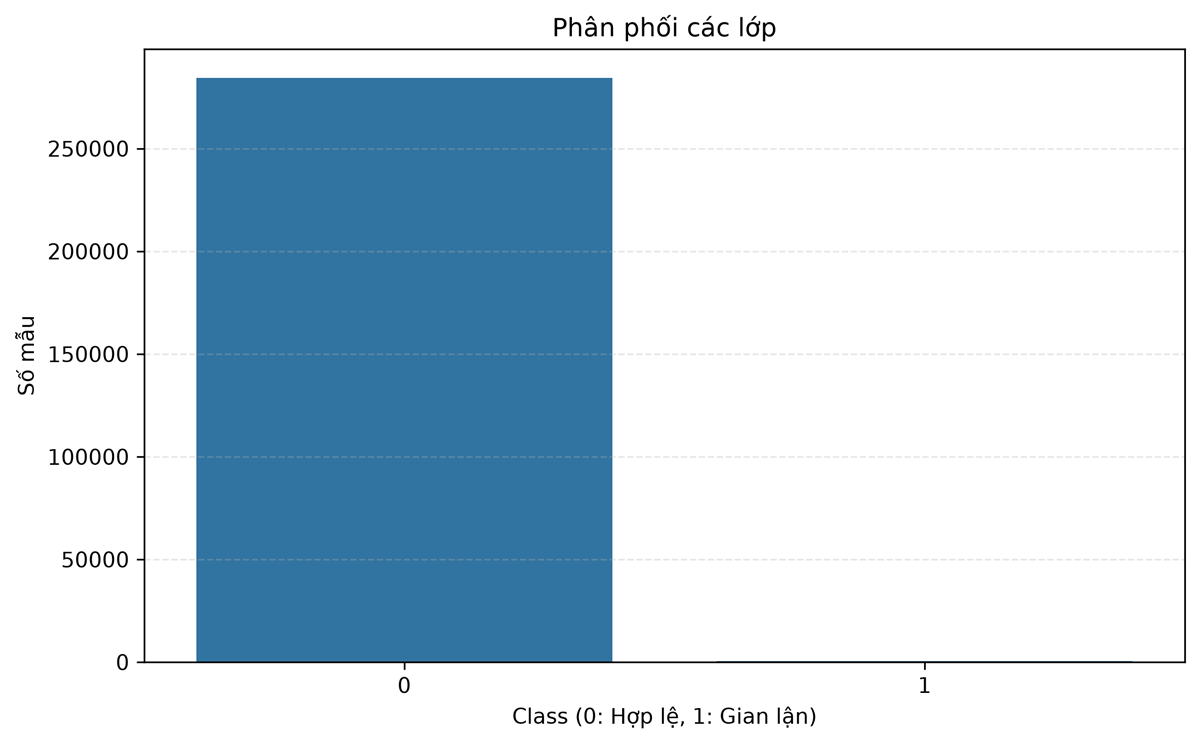
\includegraphics[width=0.58\textwidth]{class_distribution.png}
    \caption{Phân bố số giao dịch theo lớp}
    \label{fig:class-distribution}
\end{figure}

\subsection{Phân bố giá trị giao dịch và các đặc trưng}

Phân bố \texttt{Amount} lệch phải mạnh ở cả hai lớp. Giao dịch gian lận có giá trị trung bình khoảng 122,21 nhưng trung vị chỉ 9,25; giao dịch hợp lệ có giá trị trung bình khoảng 88,29 và trung vị 22,00. Điều này cho thấy chỉ dùng giá trị giao dịch là không đủ để phân tách hai lớp.

\begin{figure}[H]
    \centering
    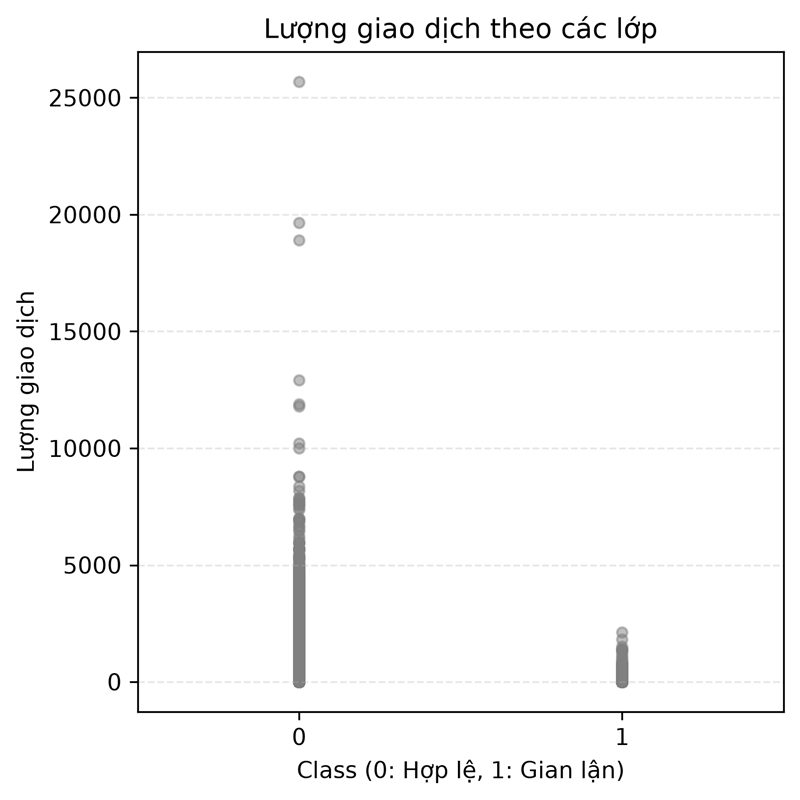
\includegraphics[width=0.42\textwidth]{transaction_amount.png}
    \caption{Phân bố giá trị giao dịch theo lớp}
    \label{fig:transaction-amount}
\end{figure}

Ma trận tương quan ở Hình~\ref{fig:correlation} chủ yếu cho thấy tương quan tuyến tính giữa các biến. Do phần lớn đặc trưng đã qua PCA, nhiều cặp biến có tương quan thấp; tuy nhiên một số đặc trưng vẫn có quan hệ đáng chú ý với nhãn \texttt{Class}. Hình~\ref{fig:feature-distribution} bổ sung góc nhìn theo phân bố: một số biến như các thành phần PCA có hình dạng khác nhau rõ hơn giữa hai lớp và có thể đóng góp vào việc nhận diện gian lận.

\begin{figure}[H]
    \centering
    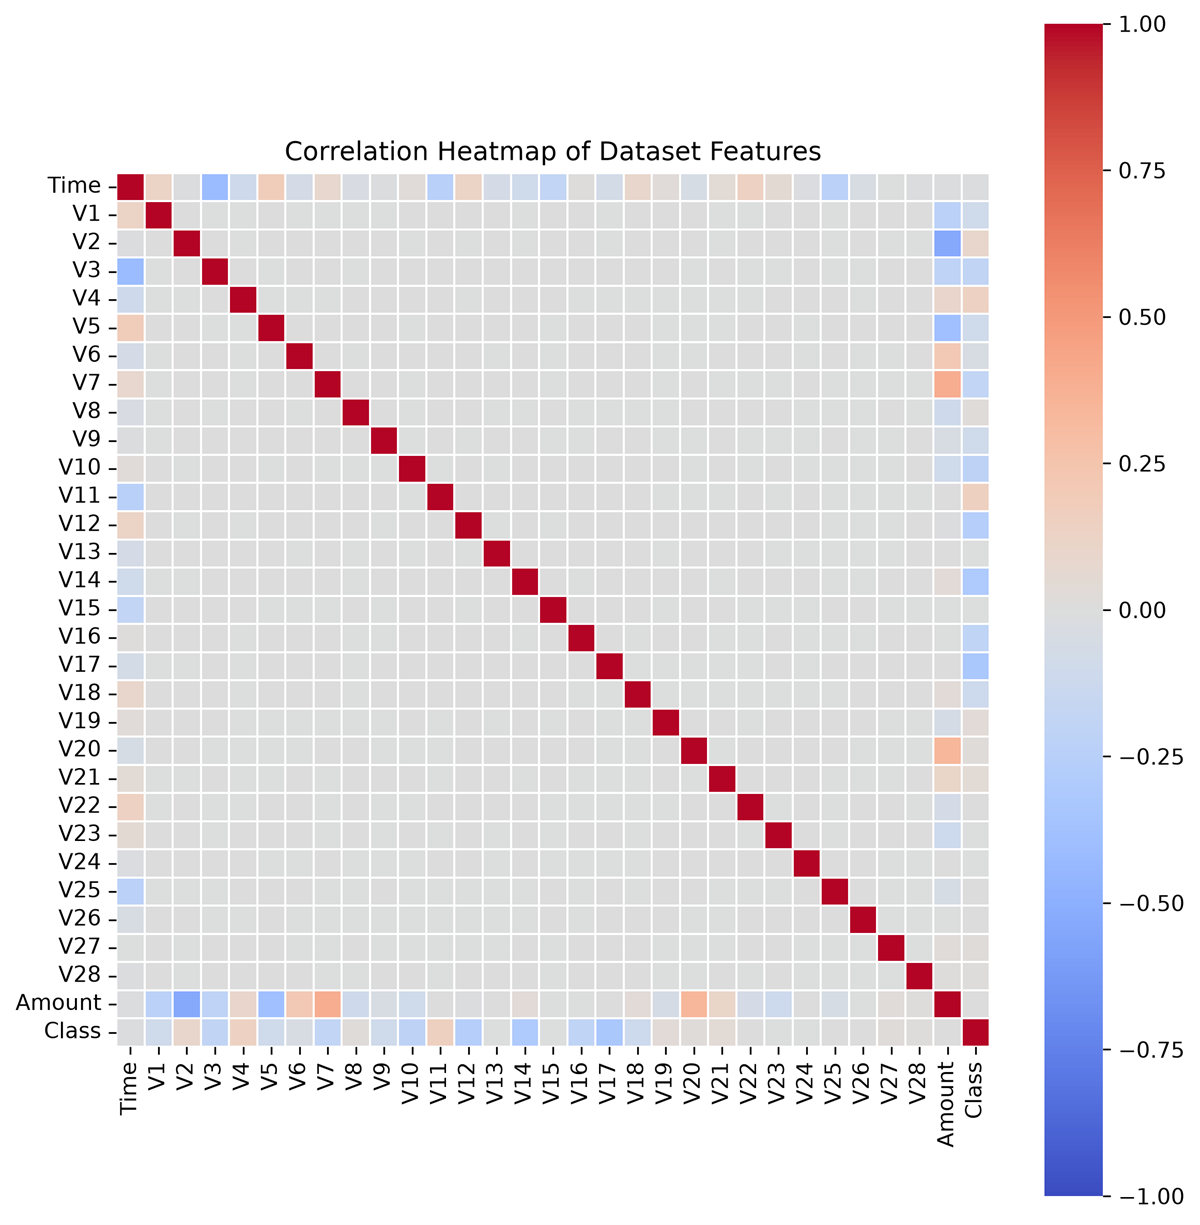
\includegraphics[width=0.67\textwidth]{correlation_matrix.png}
    \caption{Ma trận tương quan giữa các thuộc tính}
    \label{fig:correlation}
\end{figure}

\begin{figure}[H]
    \centering
    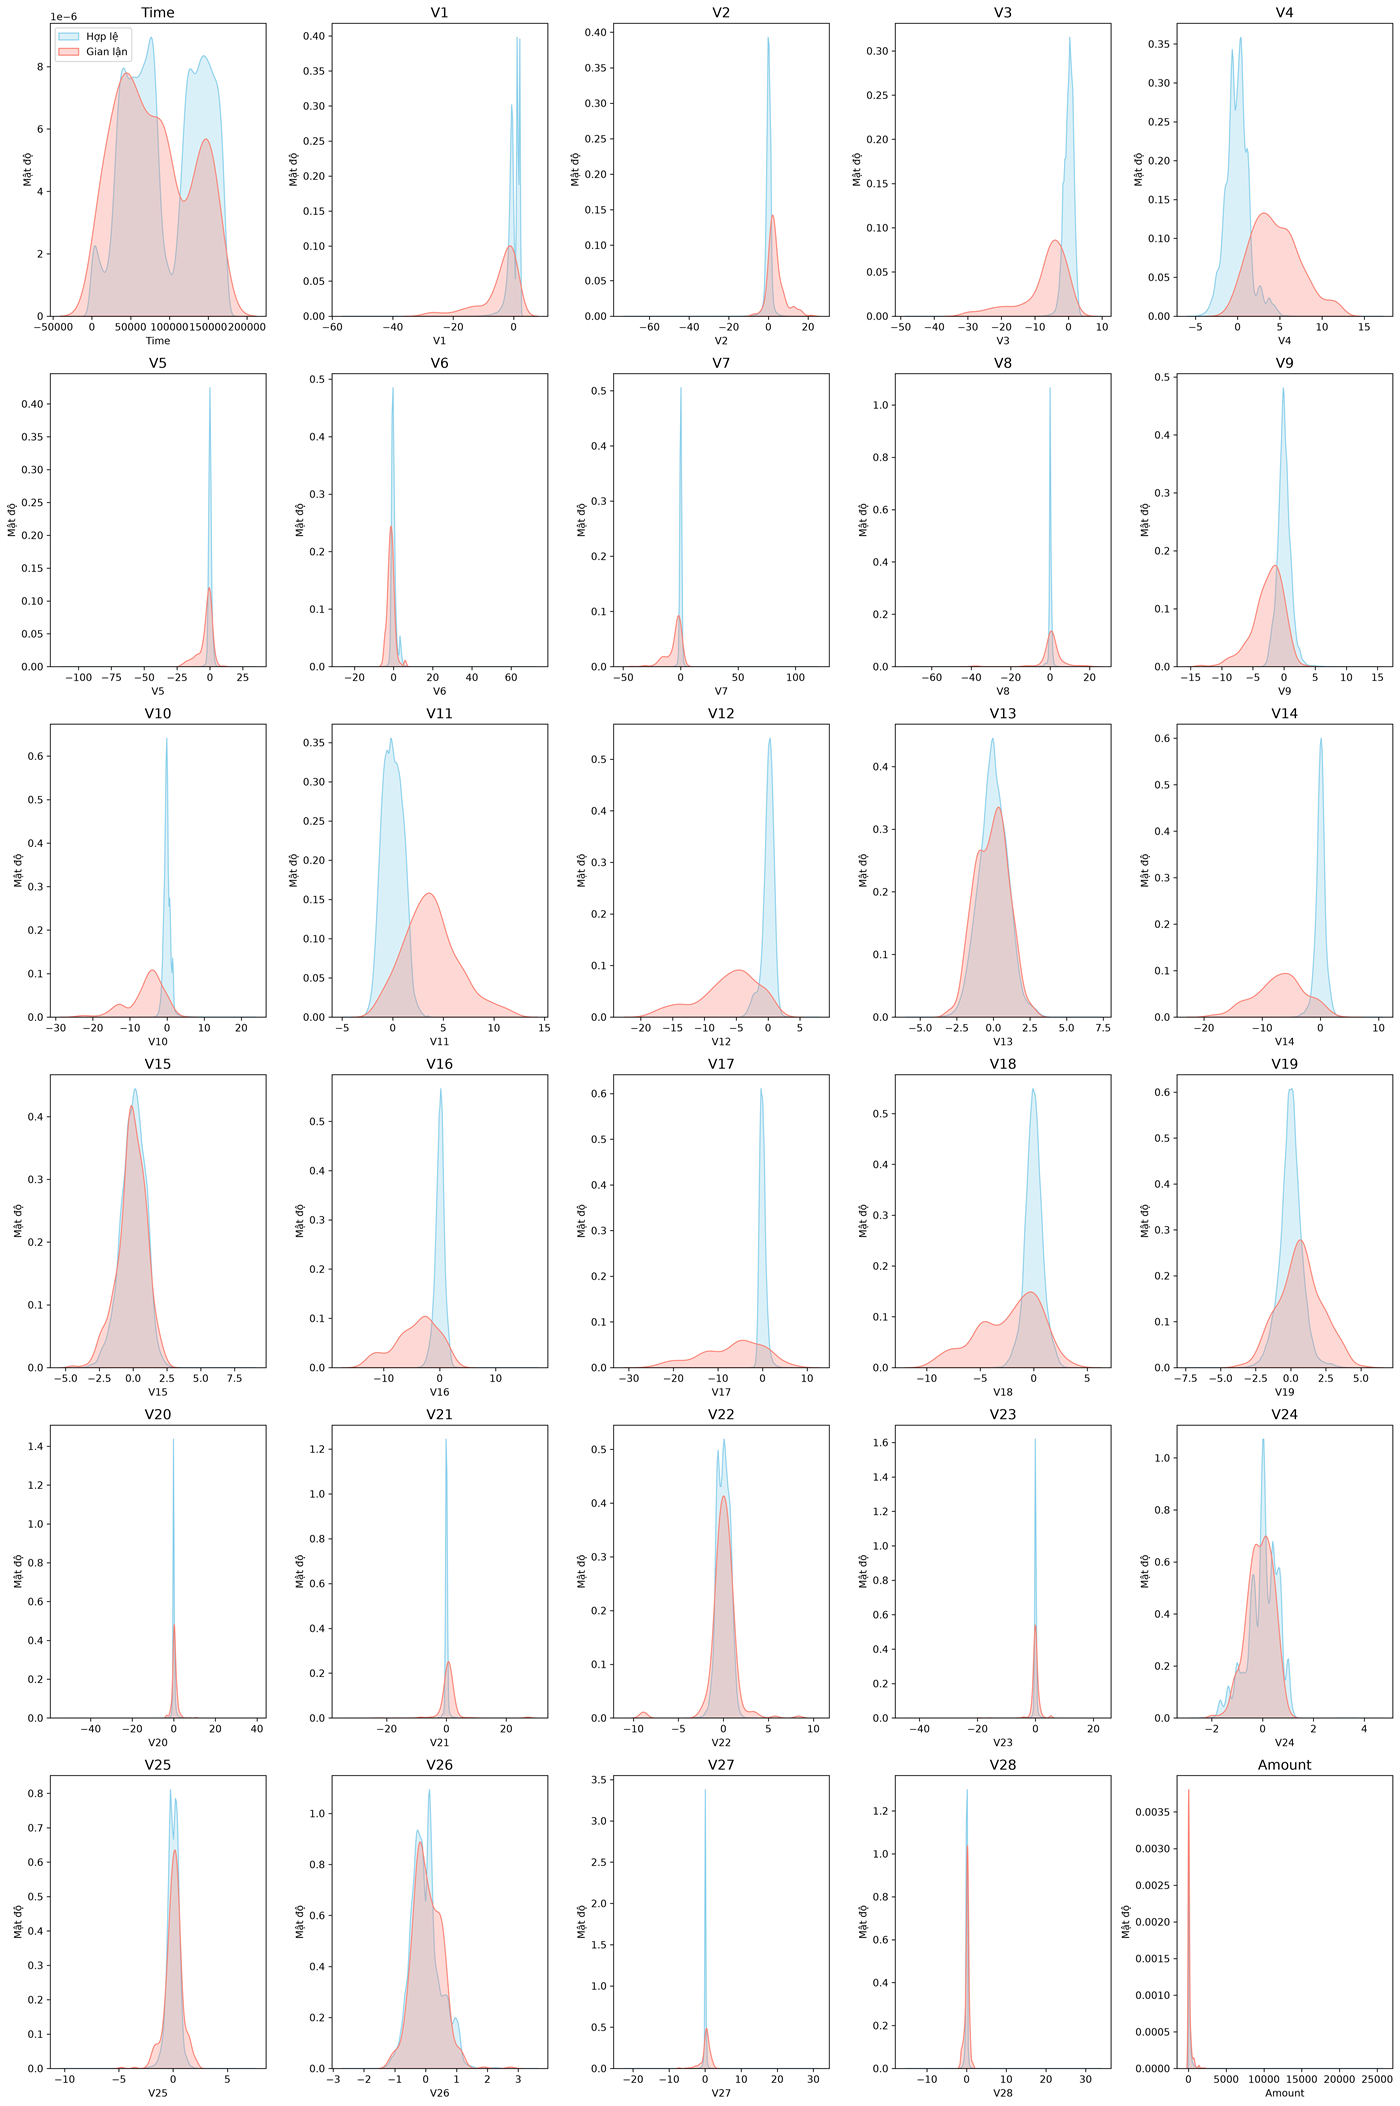
\includegraphics[width=0.98\textwidth]{feature_distribution.png}
    \caption{Phân bố các đặc trưng của lớp hợp lệ và lớp gian lận}
    \label{fig:feature-distribution}
\end{figure}

\section{Phương pháp nghiên cứu}

\subsection{Quy trình thực nghiệm}

Quy trình được thực hiện theo thứ tự sau:
\begin{enumerate}
    \item Tách \texttt{Class} khỏi tập đặc trưng.
    \item Chia dữ liệu thành 80\% train và 20\% test bằng \texttt{train\_test\_split}, sử dụng \texttt{stratify=y}, \texttt{shuffle=True} và \texttt{random\_state=42} để duy trì tỷ lệ lớp.
    \item Fit \texttt{StandardScaler} chỉ trên tập train, sau đó dùng cùng scaler để biến đổi train và test. Việc này đặc biệt cần thiết cho LR và các phương pháp dựa trên khoảng cách như Borderline-SMOTE.
    \item Áp dụng từng kỹ thuật sampling chỉ trên tập train đã chuẩn hóa. Tập test được giữ nguyên phân bố thực tế.
    \item Huấn luyện LR và XGBoost trên từng tập train sau sampling, sau đó đánh giá trên cùng một tập test với ngưỡng 0.5.
\end{enumerate}

Cách tổ chức này ngăn dữ liệu kiểm tra tham gia trực tiếp vào bước chuẩn hóa và sampling, nhờ đó giảm nguy cơ data leakage. Tuy nhiên, các phương pháp sinh dữ liệu vẫn có tính ngẫu nhiên; vì vậy kết quả có thể thay đổi nhẹ giữa các lần chạy nếu không cố định toàn bộ nguồn ngẫu nhiên.

\subsection{Các kỹ thuật xử lý mất cân bằng}

\subsubsection{Random Undersampling}

Random Undersampling loại ngẫu nhiên giao dịch thuộc lớp đa số cho đến khi số mẫu của hai lớp cân bằng. Ưu điểm là giảm thời gian huấn luyện và không tạo dữ liệu giả. Nhược điểm quan trọng là loại bỏ phần lớn giao dịch hợp lệ, khiến mô hình mất thông tin về sự đa dạng của lớp 0 và dễ tạo nhiều cảnh báo sai.

\subsubsection{Borderline-SMOTE}

Borderline-SMOTE chỉ tập trung sinh thêm các điểm thiểu số nằm gần ranh giới giữa hai lớp \cite{han2005}. Mẫu mới được nội suy từ các láng giềng thiểu số. Phương pháp này giữ lại lớp đa số và tăng thông tin gần vùng khó phân loại, nhưng có thể khuếch đại nhiễu nếu các điểm biên không đại diện tốt.

\subsubsection{CTGAN}

CTGAN là mô hình sinh dữ liệu dạng bảng dựa trên GAN có điều kiện. Generator tạo mẫu tổng hợp, còn discriminator học phân biệt mẫu thật và mẫu sinh. Cơ chế điều kiện giúp mô hình xử lý tốt hơn các cột rời rạc mất cân bằng và phân bố liên tục đa mode \cite{xu2019}. Trong project, CTGAN được fit trên các giao dịch gian lận thuộc tập train và sinh đủ mẫu lớp 1 để cân bằng với lớp 0.

\subsubsection{TVAE}

TVAE là biến thể Variational Autoencoder cho dữ liệu bảng. Encoder ánh xạ dữ liệu vào phân bố trong không gian tiềm ẩn, còn decoder tái tạo và sinh các mẫu mới. Khác với nội suy của SMOTE, TVAE học một phân bố xác suất của lớp gian lận, nhưng chất lượng mẫu phụ thuộc mạnh vào số lượng mẫu thật và cấu hình huấn luyện \cite{xu2019}.

\subsection{Mô hình phân loại}

\subsubsection{Logistic Regression}

LR được sử dụng làm baseline. Sau khi chuẩn hóa, mô hình ước lượng xác suất gian lận bằng hàm sigmoid:
\begin{equation}
    P(y=1\mid x)=\frac{1}{1+\exp[-(w^Tx+b)]}.
\end{equation}
Mô hình dùng \texttt{max\_iter=1000}, \texttt{random\_state=42} và ngưỡng phân loại 0.5. LR dễ huấn luyện và ổn định, nhưng biên quyết định tuyến tính có thể không biểu diễn đầy đủ quan hệ phức tạp giữa các đặc trưng.

\subsubsection{XGBoost}

XGBoost kết hợp nhiều cây quyết định theo hướng boosting. Ở vòng thứ $t$, một cây mới được thêm để sửa phần sai số của mô hình trước đó. Dự đoán của mô hình có dạng:
\begin{equation}
    \hat{y}_i=\sum_{k=1}^{K} f_k(x_i), \qquad f_k\in\mathcal{F}.
\end{equation}

Sau khi phân tích learning curve, cấu hình cũ có bước học lớn được thay bằng cấu hình regularization mạnh hơn nhằm giảm dao động và overfitting. Các tham số cuối cùng được trình bày trong Bảng~\ref{tab:xgb-params}.

\begin{table}[H]
    \centering
    \begin{tabular}{llll}
        \toprule
        \textbf{Tham số} & \textbf{Giá trị} & \textbf{Tham số} & \textbf{Giá trị} \\
        \midrule
        \texttt{objective} & \texttt{binary:logistic} & \texttt{eval\_metric} & \texttt{logloss} \\
        \texttt{learning\_rate} & 0.05 & \texttt{n\_estimators} & 400 \\
        \texttt{max\_depth} & 4 & \texttt{min\_child\_weight} & 5 \\
        \texttt{subsample} & 0.8 & \texttt{colsample\_bytree} & 0.8 \\
        \texttt{gamma} & 0.1 & \texttt{reg\_alpha} & 0.1 \\
        \texttt{reg\_lambda} & 5 & \texttt{tree\_method} & \texttt{hist} \\
        \texttt{random\_state} & 42 & Ngưỡng phân loại & 0.5 \\
        \bottomrule
    \end{tabular}
    \caption{Cấu hình XGBoost sử dụng trong thực nghiệm}
    \label{tab:xgb-params}
\end{table}

\section{Thiết kế đánh giá}

\subsection{Các chỉ số}

Gọi TP là số gian lận được phát hiện đúng, TN là số giao dịch hợp lệ được dự đoán đúng, FP là giao dịch hợp lệ bị cảnh báo nhầm và FN là gian lận bị bỏ sót. Các chỉ số được tính như sau:
\begin{align}
    \text{Accuracy} &= \frac{TP+TN}{TP+TN+FP+FN},\\
    \text{Precision} &= \frac{TP}{TP+FP},\\
    \text{Recall} &= \frac{TP}{TP+FN},\\
    \text{F1} &= 2\frac{\text{Precision}\times\text{Recall}}
    {\text{Precision}+\text{Recall}}.
\end{align}

Precision cho biết mức độ đáng tin của một cảnh báo gian lận; Recall cho biết tỷ lệ gian lận thực tế được phát hiện. F1-score là trung bình điều hòa của hai chỉ số và được dùng làm tiêu chí so sánh chính. Accuracy vẫn được báo cáo nhưng không dùng để kết luận độc lập vì lớp hợp lệ chiếm ưu thế tuyệt đối.

\subsection{Learning curve}

Learning curve được tính trên dữ liệu train gốc trước sampling. Với mỗi tỷ lệ từ 10\% đến 100\%, mô hình được đánh giá bằng cả F1-score và Recall qua Stratified 5-fold Cross-Validation có xáo trộn và \texttt{random\_state=42}. Đường training phản ánh mức độ khớp dữ liệu huấn luyện, đường validation phản ánh khả năng khái quát; vùng mờ biểu diễn độ lệch chuẩn giữa các fold. Hai chỉ số cần được xem đồng thời: F1 đo sự cân bằng giữa Precision và Recall, còn Recall tập trung trực tiếp vào tỷ lệ gian lận được phát hiện.

\begin{figure}[H]
    \centering
    \begin{minipage}{0.49\textwidth}
        \centering
        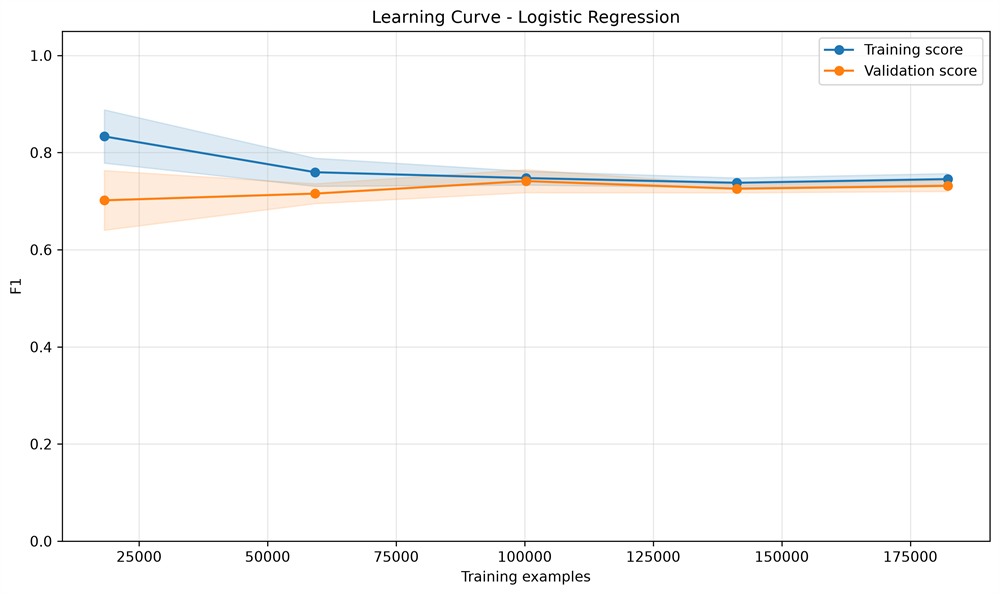
\includegraphics[width=\linewidth]{learning_curve_logistic_regression.png}
        \caption{F1 learning curve của Logistic Regression}
        \label{fig:lc-lr}
    \end{minipage}\hfill
    \begin{minipage}{0.49\textwidth}
        \centering
        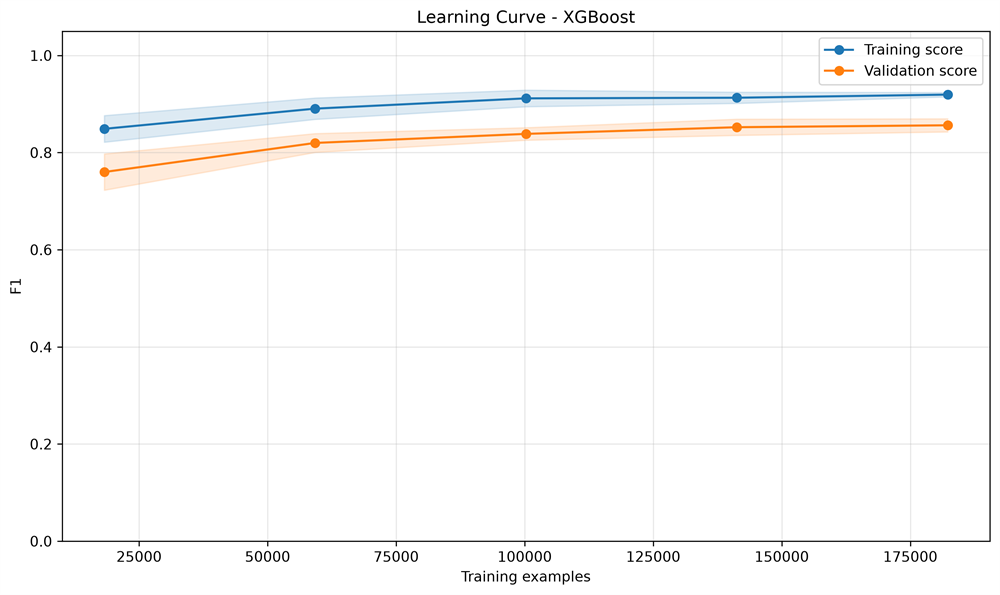
\includegraphics[width=\linewidth]{learning_curve_xgboost.png}
        \caption{F1 learning curve của XGBoost}
        \label{fig:lc-xgb}
    \end{minipage}
\end{figure}

Ở LR, training F1 giảm khi số mẫu tăng, validation F1 tăng nhẹ rồi hai đường hội tụ quanh 0,73--0,75. Khoảng cách nhỏ và độ lệch chuẩn thu hẹp cho thấy mô hình ổn định, ít overfit, nhưng mức F1 sớm bão hòa phản ánh giới hạn của biên quyết định tuyến tính và dấu hiệu high bias.

Với XGBoost, training F1 tăng từ khoảng 0,85 lên trên 0,90, trong khi validation F1 tăng từ khoảng 0,76 lên khoảng 0,85. Hai đường không hội tụ hoàn toàn nên mô hình vẫn có variance nhất định, nhưng khoảng cách nhỏ hơn nhiều so với cấu hình cũ và các vùng độ lệch chuẩn thu hẹp khi dữ liệu tăng. Điều này cho thấy việc giảm bước học, giới hạn độ sâu cây và thêm regularization đã giúp mô hình học ổn định hơn.

\begin{figure}[H]
    \centering
    \begin{minipage}{0.49\textwidth}
        \centering
        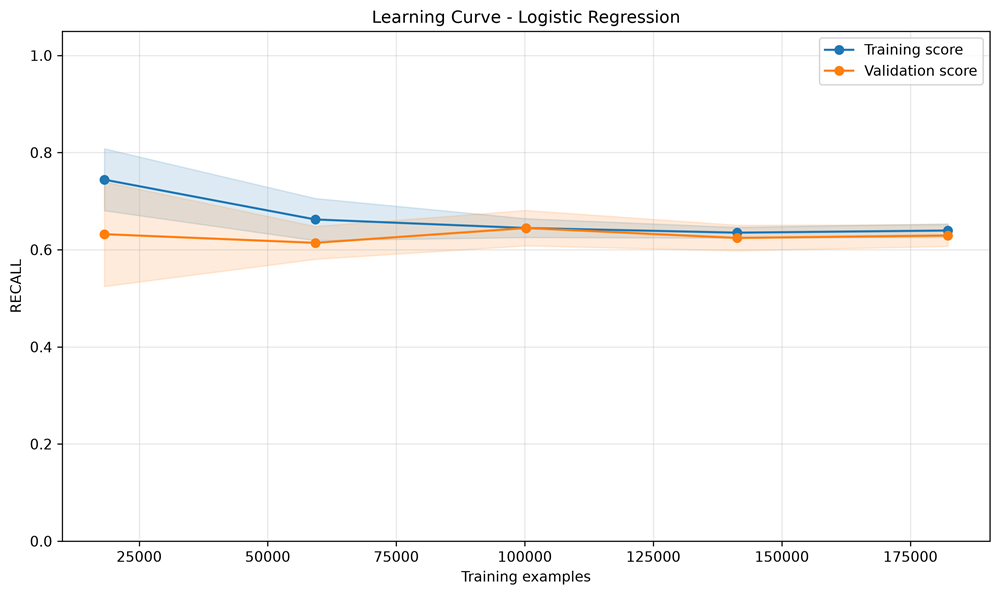
\includegraphics[width=\linewidth]{learning_curve_logistic_regression_recall.png}
        \caption{Recall learning curve của Logistic Regression}
        \label{fig:lc-recall-lr}
    \end{minipage}\hfill
    \begin{minipage}{0.49\textwidth}
        \centering
        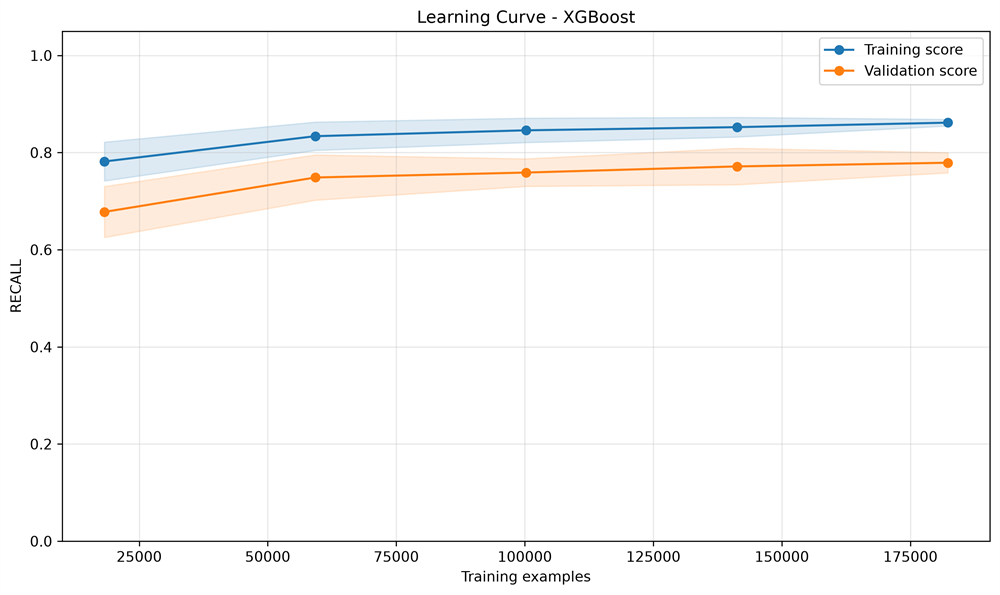
\includegraphics[width=\linewidth]{learning_curve_xgboost_recall.png}
        \caption{Recall learning curve của XGBoost}
        \label{fig:lc-recall-xgb}
    \end{minipage}
\end{figure}

Recall learning curve làm rõ một hạn chế mà F1 chưa thể hiện đầy đủ. Với LR, training Recall giảm từ 0,744 xuống 0,640 và validation Recall hội tụ quanh 0,629. Hai đường gần nhau cho thấy kết quả ổn định, nhưng mô hình chỉ phát hiện được khoảng 63\% số giao dịch gian lận ở ngưỡng 0.5. Nói cách khác, F1 khoảng 0,73 không đồng nghĩa LR đã bắt được phần lớn fraud; mô hình đạt F1 tương đối khá nhờ Precision cao nhưng vẫn bỏ sót nhiều mẫu dương.

Với XGBoost, validation Recall tăng từ 0,678 lên 0,779 khi số mẫu huấn luyện tăng, trong khi training Recall cuối đạt khoảng 0,862. XGBoost phát hiện fraud tốt hơn LR, nhưng validation Recall vẫn thấp hơn F1 validation. Khoảng cách khoảng 0,08 giữa train và validation cho thấy mô hình vẫn còn variance và còn dư địa cải thiện khả năng phát hiện lớp thiểu số. Đây là cơ sở để khảo sát sampling theo mục tiêu tăng Recall, thay vì giả định sampling nhất thiết phải làm F1 cao hơn.

\section{Kết quả và thảo luận}

\subsection{Kết quả tổng hợp}

Bảng~\ref{tab:results} trình bày kết quả trên tập test giữ nguyên phân bố ban đầu. Hai hàng ``Không sampling'' là nhóm đối chứng: mô hình được huấn luyện trực tiếp trên tập train gốc đã chuẩn hóa. Các hàng còn lại chỉ thay đổi dữ liệu huấn luyện bằng từng kỹ thuật sampling. Tất cả cấu hình sử dụng cùng tập test và ngưỡng 0.5, vì vậy đây là phép so sánh trực tiếp hơn so với việc đối chiếu learning curve cross-validation với điểm test.

\begin{table}[H]
    \centering
    \small
    \setlength{\tabcolsep}{4.2pt}
    \begin{tabular}{llrrrr}
        \toprule
        \textbf{Sampling} & \textbf{Mô hình} & \textbf{Accuracy} & \textbf{Precision} & \textbf{Recall} & \textbf{F1} \\
        \midrule
        Không sampling & LR & 99,91\% & 82,67\% & 63,27\% & 71,68\% \\
        Không sampling & XGBoost & \textbf{99,96\%} & \textbf{93,02\%} & 81,63\% & \textbf{86,96\%} \\
        \midrule
        Undersampling & LR & 96,02\% & 3,83\% & \textbf{91,84\%} & 7,36\% \\
        Undersampling & XGBoost & 95,72\% & 3,57\% & \textbf{91,84\%} & 6,87\% \\
        \midrule
        Borderline-SMOTE & LR & 98,66\% & 10,16\% & 86,73\% & 18,18\% \\
        Borderline-SMOTE & XGBoost & 99,92\% & 73,68\% & 85,71\% & 79,25\% \\
        \midrule
        CTGAN & LR & 99,91\% & 71,30\% & 83,67\% & 77,00\% \\
        CTGAN & XGBoost & 99,94\% & 79,61\% & 83,67\% & 81,59\% \\
        \midrule
        TVAE & LR & 99,82\% & 49,40\% & 84,69\% & 62,41\% \\
        TVAE & XGBoost & 99,94\% & 84,04\% & 80,61\% & 82,29\% \\
        \bottomrule
    \end{tabular}
    \caption{Kết quả của LR và XGBoost trước và sau sampling}
    \label{tab:results}
\end{table}

\subsection{Tác động của sampling đến Recall}

So với baseline không sampling, sampling làm Recall của LR tăng ở cả bốn phương pháp. Mức tăng dao động từ 20,40 đến 28,57 điểm phần trăm. Đối với XGBoost, ba phương pháp Undersampling, Borderline-SMOTE và CTGAN làm Recall tăng; riêng TVAE làm Recall giảm nhẹ 1,02 điểm phần trăm. Vì vậy, nhận định chính xác không phải là sampling luôn cải thiện Recall, mà là sampling nhìn chung dịch chuyển mô hình về phía ưu tiên phát hiện lớp gian lận, với mức độ phụ thuộc vào mô hình và cách tạo mẫu.

\begin{table}[H]
    \centering
    \begin{tabular}{lrr}
        \toprule
        \textbf{Sampling} & \textbf{$\Delta$ Recall LR} & \textbf{$\Delta$ Recall XGBoost} \\
        \midrule
        Undersampling & +28,57 điểm \% & +10,21 điểm \% \\
        Borderline-SMOTE & +23,46 điểm \% & +4,08 điểm \% \\
        CTGAN & +20,40 điểm \% & +2,04 điểm \% \\
        TVAE & +21,42 điểm \% & -1,02 điểm \% \\
        \bottomrule
    \end{tabular}
    \caption{Thay đổi Recall so với mô hình không sampling trên cùng tập test}
    \label{tab:recall-change}
\end{table}

Kết quả này cho thấy sampling có ý nghĩa nếu mục tiêu nghiệp vụ ưu tiên giảm FN. Tuy nhiên, Recall tăng không đồng nghĩa mô hình tốt hơn trên mọi phương diện. Sampling thay đổi phân bố lớp trong tập train và khiến mô hình dự đoán class 1 thường xuyên hơn; do đó TP có thể tăng nhưng FP cũng tăng. F1 chỉ tăng khi lợi ích từ Recall đủ lớn để bù cho phần Precision bị mất. Đây là lý do LR + CTGAN cải thiện cả Recall và F1, trong khi phần lớn cấu hình XGBoost sau sampling có Recall cao hơn nhưng F1 thấp hơn baseline.

\subsection{Phân tích theo kỹ thuật sampling}

Trước sampling, tập train có 227.451 mẫu hợp lệ và 394 mẫu gian lận, tương ứng tỷ lệ xấp xỉ 577:1. Các hàm sampling trong project đều đưa hai lớp về gần tỷ lệ 1:1. Vì vậy, sampling không chỉ làm tăng số mẫu lớp thiểu số mà còn thay đổi mạnh xác suất tiên nghiệm mà mô hình quan sát trong lúc huấn luyện. Khi đánh giá trên tập test vẫn giữ tỷ lệ gian lận tự nhiên rất thấp, mô hình sau sampling thường nhạy hơn với class 1: số TP có thể tăng nhưng số FP cũng dễ tăng. Mức độ đánh đổi này khác nhau giữa từng kỹ thuật và từng mô hình.

\textbf{Undersampling.} Phương pháp này loại 227.057 mẫu hợp lệ và chỉ giữ lại 394 mẫu của mỗi lớp, làm tập train giảm xuống còn 788 quan sát. Cả LR và XGBoost nhờ đó ít bị chi phối bởi lớp 0 hơn và phát hiện đúng 90 trong tổng số 98 giao dịch gian lận trên test, tương ứng Recall 91,84\%. Tuy nhiên, Precision giảm xuống dưới 4\%, dẫn đến F1 dưới 8\%. LR cảnh báo nhầm 2.258 giao dịch hợp lệ, còn XGBoost cảnh báo nhầm 2.431 giao dịch. Nguyên nhân chính là mô hình chỉ được quan sát một phần rất nhỏ không gian phân bố của lớp hợp lệ; nhiều mẫu hợp lệ trên test trở nên khác với những gì mô hình đã học và bị đẩy sang class 1. Nói cách khác, Undersampling giảm thiên lệch về lớp đa số nhưng đồng thời làm tăng variance và làm mất nhiều thông tin quan trọng về lớp 0. Đây là ví dụ rõ nhất cho việc Recall cao không đồng nghĩa mô hình có chất lượng tổng thể tốt.

\textbf{Borderline-SMOTE.} Thay vì loại lớp đa số, Borderline-SMOTE giữ lại các giao dịch hợp lệ và sinh mẫu fraud mới quanh những điểm thiểu số nằm gần ranh giới phân lớp. Cách làm này tăng mật độ class 1 tại vùng khó phân biệt, khiến biên quyết định dịch về phía lớp hợp lệ và giúp Recall tăng lên 86,73\% với LR và 85,71\% với XGBoost. Tuy nhiên, các mẫu nội suy gần biên cũng có thể chồng lấn với phân bố lớp 0 hoặc khuếch đại những điểm fraud nhiễu. Ảnh hưởng này đặc biệt rõ với LR: mô hình chỉ có một biên tuyến tính nên sự dịch chuyển của biên làm xuất hiện 752 FP, khiến Precision chỉ còn 10,16\% và F1 đạt 18,18\%. XGBoost có khả năng tạo nhiều vùng phân tách phi tuyến nên kiểm soát vùng chồng lấn tốt hơn, chỉ tạo 30 FP và đạt F1 79,25\%. Dù vậy, Precision 73,68\% vẫn thấp hơn baseline 93,02\%, cho thấy bốn điểm phần trăm Recall tăng thêm phải đánh đổi bằng số cảnh báo sai lớn hơn.

\textbf{CTGAN.} CTGAN không nội suy trực tiếp giữa các điểm fraud mà học phân bố kết hợp của các đặc trưng rồi sinh giao dịch mới từ phân bố đó. Nhờ tạo ra các tổ hợp đặc trưng đa dạng hơn, CTGAN giúp LR mở rộng vùng nhận diện class 1: số fraud phát hiện đúng tăng từ 62 lên 82, FN giảm từ 36 xuống 16. Mặc dù FP tăng từ 13 lên 33 và Precision giảm từ 82,67\% xuống 71,30\%, phần Recall tăng từ 63,27\% lên 83,67\% đủ lớn để F1 tăng từ 71,68\% lên 77,00\%. Đây là trường hợp duy nhất trong thí nghiệm mà sampling làm F1 tốt hơn baseline tương ứng. Với XGBoost, CTGAN cũng làm TP tăng từ 80 lên 82 và Recall tăng 2,04 điểm phần trăm, nhưng FP tăng từ 6 lên 21. Vì Precision giảm từ 93,02\% xuống 79,61\%, F1 còn 81,59\%, thấp hơn mức 86,96\% của baseline. Một nguyên nhân có thể là XGBoost vốn đã học tốt cấu trúc fraud thật nên lợi ích từ hai TP bổ sung không đủ bù cho các FP phát sinh. Đồng thời, CTGAN chỉ được fit từ 394 fraud thật nhưng phải sinh một lượng dữ liệu rất lớn; nếu dữ liệu sinh chứa đặc trưng chưa sát phân bố thật, mô hình cây có thể học cả các quy luật nhân tạo không khái quát tốt trên test.

\textbf{TVAE.} TVAE mã hóa các giao dịch fraud vào không gian tiềm ẩn và sinh mẫu thông qua decoder. Cơ chế tái tạo thường tạo phân bố trơn hơn, có thể bao phủ các vùng trung tâm của lớp fraud nhưng làm mờ một số cấu trúc hiếm hoặc ranh giới phức tạp. Với LR, số TP tăng từ 62 lên 83 nhưng FP tăng mạnh từ 13 lên 85. Recall vì thế tăng từ 63,27\% lên 84,69\%, trong khi Precision chỉ còn 49,40\% và F1 giảm xuống 62,41\%. Với XGBoost, TVAE tạo ít FP nhất trong nhóm có sampling, chỉ 15 trường hợp, nên Precision đạt 84,04\% và F1 đạt 82,29\%, cao nhất trong riêng nhóm sampling. Tuy nhiên, mô hình chỉ phát hiện đúng 79 fraud, thấp hơn baseline một trường hợp, nên Recall giảm còn 80,61\%. Kết quả này gợi ý các mẫu TVAE giúp XGBoost giữ biên quyết định tương đối thận trọng nhưng chưa bổ sung được những kiểu fraud mới mà baseline bỏ sót.

Nhìn chung, sampling trong thí nghiệm này chủ yếu làm thay đổi sự đánh đổi giữa FN và FP chứ không bảo đảm làm mô hình tốt hơn theo mọi chỉ số. Việc cân bằng hoàn toàn về 1:1 khiến class fraud được nhấn mạnh mạnh hơn nhiều so với tỷ lệ thật trên test; kết hợp với ngưỡng 0.5 cố định, mô hình có xu hướng dự đoán class 1 thường xuyên hơn. LR hưởng lợi rõ nhất từ CTGAN vì baseline của mô hình còn bỏ sót nhiều fraud, trong khi XGBoost baseline đã có Precision và F1 cao nên phần Recall tăng thêm từ sampling không đủ bù cho Precision bị mất. Do đó, giá trị của sampling cần được đánh giá theo mục tiêu nghiệp vụ: nếu ưu tiên giảm FN thì một số phương pháp vẫn hữu ích, còn nếu ưu tiên F1 hoặc hạn chế cảnh báo sai thì baseline không sampling có thể phù hợp hơn.

\subsection{Confusion matrix}

Các confusion matrix của LR được trình bày trong Hình~\ref{fig:cm-lr}. Sự khác biệt lớn nhất nằm ở số FP: Undersampling và Borderline-SMOTE ưu tiên phát hiện class 1 nhưng đánh đổi bằng nhiều cảnh báo nhầm, trong khi CTGAN tạo sự cân bằng tốt hơn.

\begin{figure}[H]
    \centering
    \begin{minipage}{0.48\textwidth}
        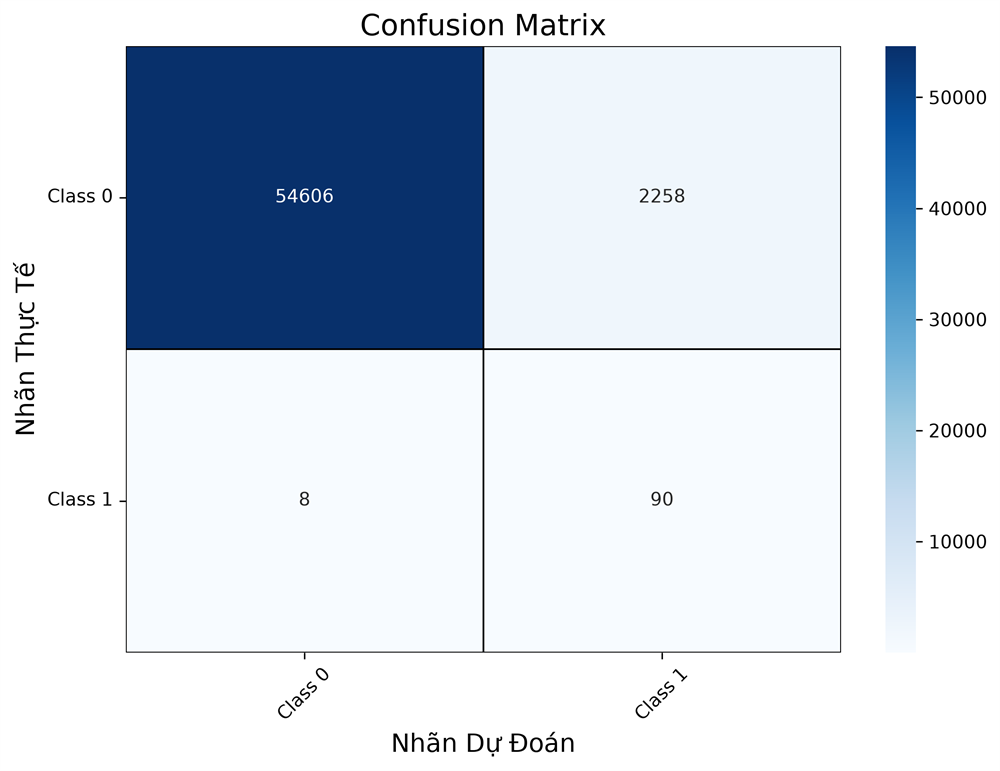
\includegraphics[width=\linewidth]{logistic_regression_undersampling.png}
    \end{minipage}\hfill
    \begin{minipage}{0.48\textwidth}
        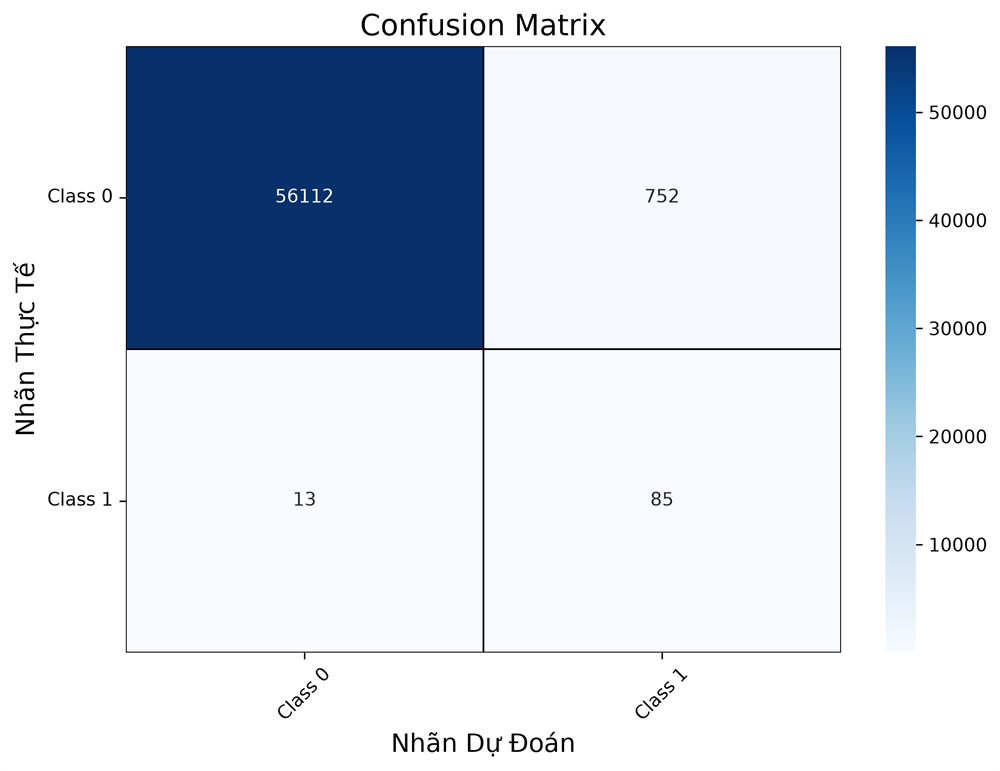
\includegraphics[width=\linewidth]{logistic_regression_oversampling.png}
    \end{minipage}

    \vspace{0.25cm}
    \begin{minipage}{0.48\textwidth}
        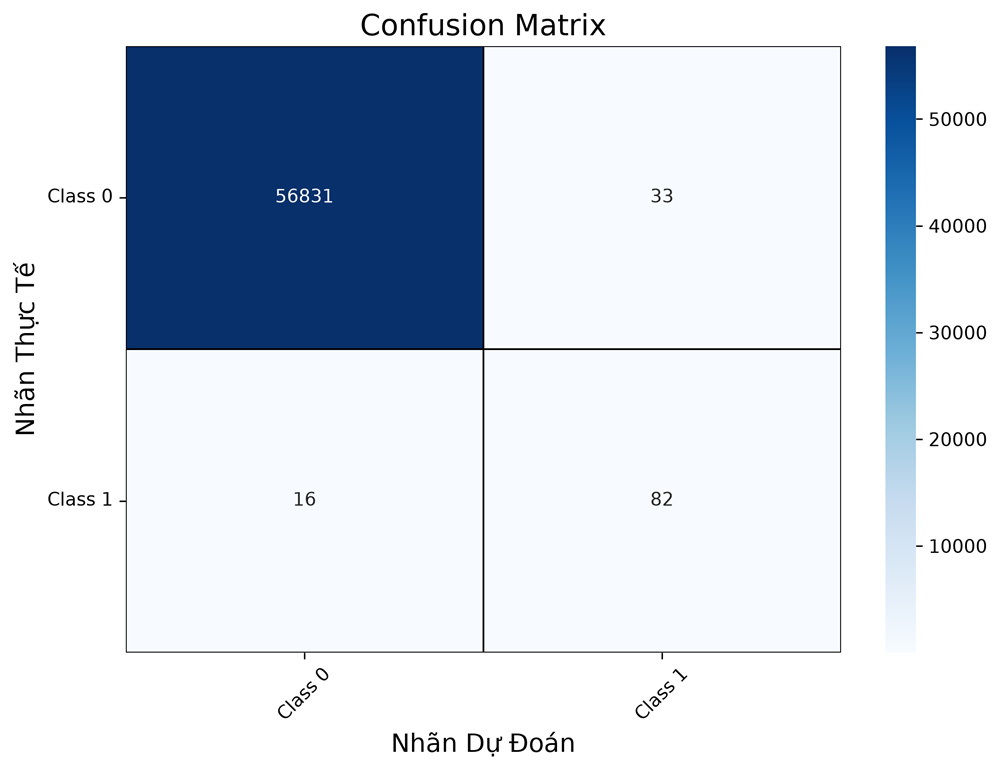
\includegraphics[width=\linewidth]{logistic_regression_ctgan.png}
    \end{minipage}\hfill
    \begin{minipage}{0.48\textwidth}
        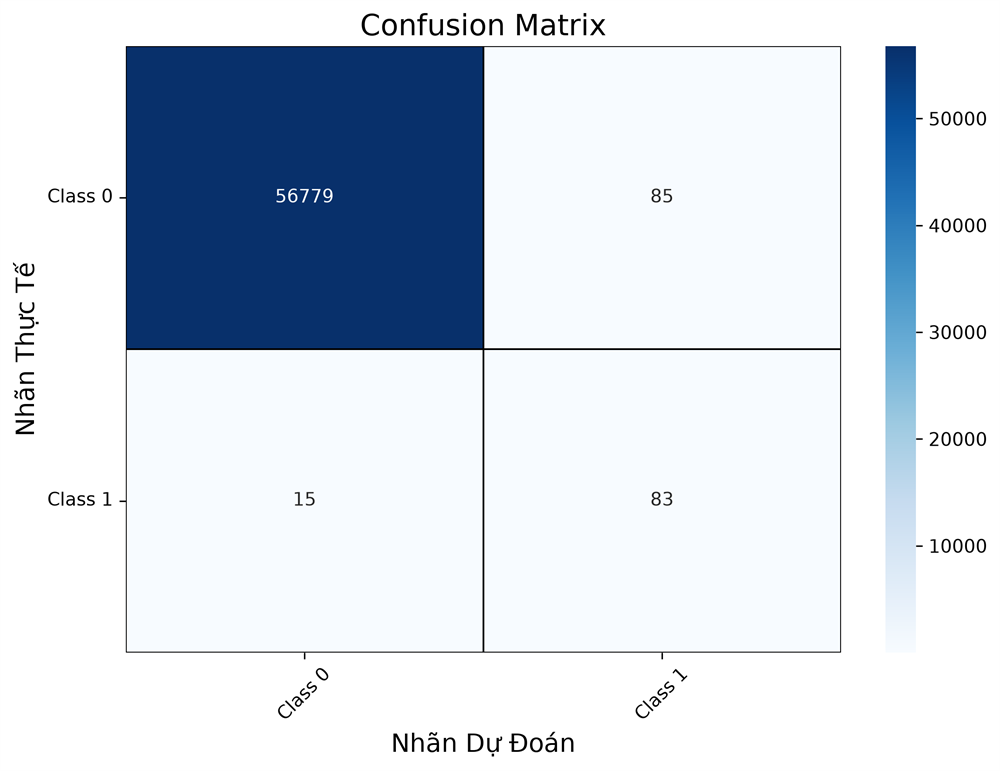
\includegraphics[width=\linewidth]{logistic_regression_tvae.png}
    \end{minipage}
    \caption{Confusion matrix của Logistic Regression: Undersampling, Borderline-SMOTE, CTGAN và TVAE theo thứ tự từ trái sang phải, từ trên xuống dưới}
    \label{fig:cm-lr}
\end{figure}

Hình~\ref{fig:cm-xgb} cho thấy XGBoost giảm FP rõ rệt khi chuyển từ Undersampling sang ba phương pháp sinh thêm dữ liệu. TVAE tạo ít FP nhất trong nhóm XGBoost nhưng bỏ sót nhiều gian lận hơn CTGAN và Borderline-SMOTE, phù hợp với sự đánh đổi Precision--Recall trong Bảng~\ref{tab:results}.

\begin{figure}[H]
    \centering
    \begin{minipage}{0.48\textwidth}
        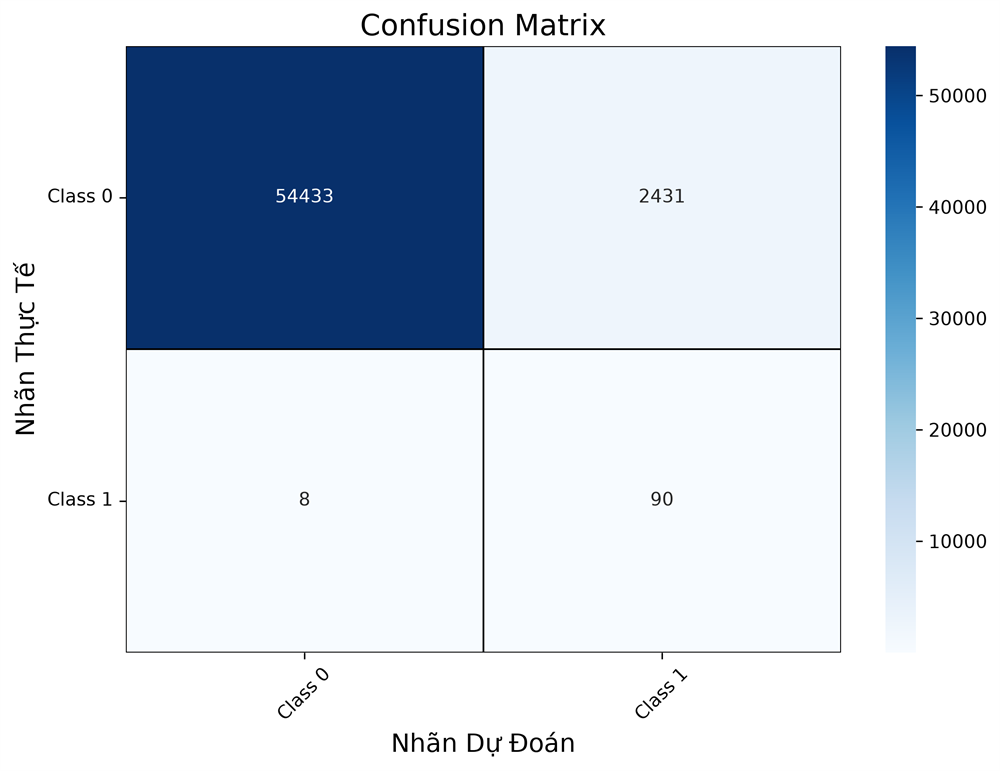
\includegraphics[width=\linewidth]{xgboost_undersampling.png}
    \end{minipage}\hfill
    \begin{minipage}{0.48\textwidth}
        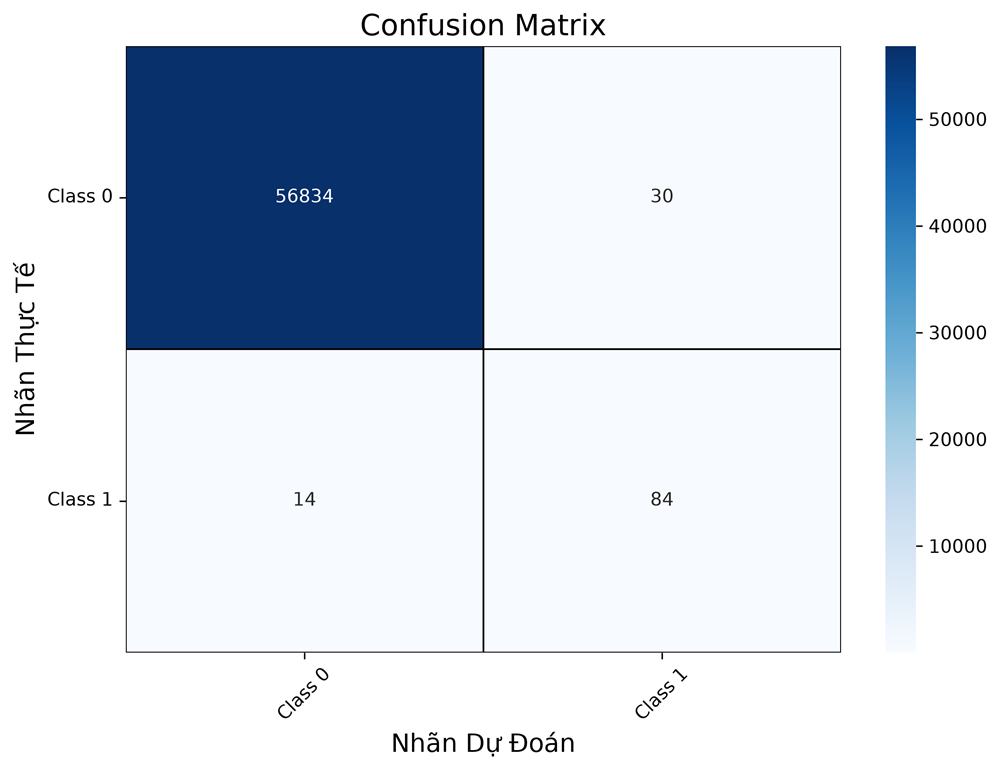
\includegraphics[width=\linewidth]{xgboost_oversampling.png}
    \end{minipage}

    \vspace{0.25cm}
    \begin{minipage}{0.48\textwidth}
        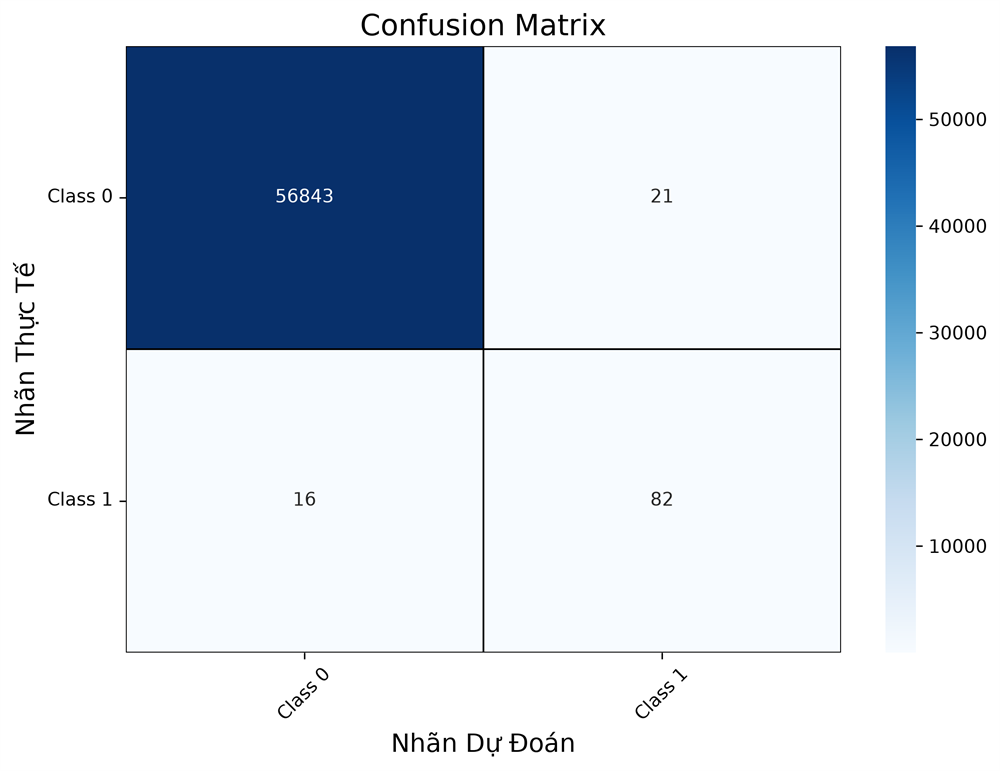
\includegraphics[width=\linewidth]{xgboost_ctgan.png}
    \end{minipage}\hfill
    \begin{minipage}{0.48\textwidth}
        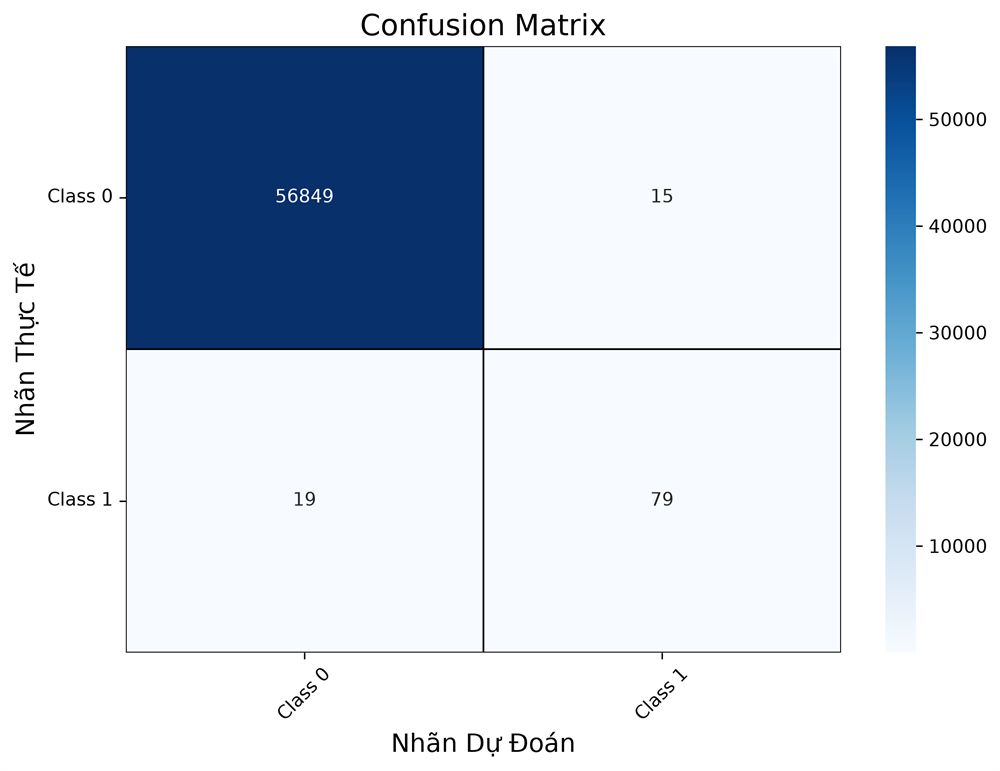
\includegraphics[width=\linewidth]{xgboost_tvae.png}
    \end{minipage}
    \caption{Confusion matrix của XGBoost: Undersampling, Borderline-SMOTE, CTGAN và TVAE theo thứ tự từ trái sang phải, từ trên xuống dưới}
    \label{fig:cm-xgb}
\end{figure}

\subsection{So sánh hai mô hình}

LR có learning curve ổn định nhưng Recall baseline chỉ đạt 63,27\% trên test, cho thấy mô hình tuyến tính còn bỏ sót nhiều fraud. Sampling có tác động rõ hơn đối với LR; đặc biệt CTGAN đồng thời nâng Recall lên 83,67\% và F1 lên 77,00\%. Đây là cấu hình duy nhất trong thí nghiệm cải thiện F1 so với baseline của chính LR.

XGBoost không sampling đã đạt Precision 93,02\%, Recall 81,63\% và F1 86,96\%, cao nhất toàn bộ thí nghiệm theo F1. Ba phương pháp Undersampling, Borderline-SMOTE và CTGAN làm Recall tăng, nhưng đều giảm Precision và F1. TVAE không tăng Recall. Như vậy, sampling vẫn có ý nghĩa đối với XGBoost khi mục tiêu là dịch chuyển mô hình về phía phát hiện nhiều fraud hơn, nhưng chưa chứng minh được lợi ích nếu tiêu chí chính là F1. Không tồn tại một cấu hình tối ưu cho mọi mục tiêu: baseline XGBoost tốt nhất theo F1 và Precision; Undersampling cao nhất theo Recall nhưng không thực dụng vì quá nhiều FP; Borderline-SMOTE và CTGAN tạo ra các phương án đánh đổi trung gian.

\section{Hạn chế của nghiên cứu}
\label{sec:limitations}

Các kết quả cần được diễn giải cùng những hạn chế sau:
\begin{itemize}
    \item Thí nghiệm sử dụng một lần chia train/test cố định. Chưa có repeated cross-validation trên toàn bộ pipeline sampling, vì vậy chưa đo đầy đủ độ biến thiên của kết quả.
    \item Borderline-SMOTE, CTGAN và TVAE có thành phần ngẫu nhiên; các lần sinh dữ liệu khác nhau có thể làm thay đổi chỉ số trên test.
    \item Bộ dữ liệu có 1.081 dòng trùng và project hiện chưa loại bỏ chúng. Nếu các dòng giống nhau xuất hiện ở cả train và test, kết quả có thể lạc quan hơn thực tế.
    \item Ngưỡng 0.5 được dùng thống nhất để bảo đảm so sánh trực tiếp, nhưng chưa được tối ưu theo chi phí FP và FN trong nghiệp vụ.
    \item Chất lượng và tính riêng tư của dữ liệu sinh bởi CTGAN/TVAE chưa được đánh giá bằng các phép đo fidelity, utility hoặc disclosure risk độc lập.
    \item Dữ liệu chỉ bao phủ hai ngày giao dịch và các đặc trưng chính đã được ẩn danh, nên chưa đánh giá được hiện tượng thay đổi hành vi gian lận theo thời gian.
\end{itemize}

\section{Kết luận}

Project đã xây dựng quy trình so sánh LR và XGBoost trên dữ liệu mất cân bằng, trong đó scaler chỉ được fit trên tập train và sampling chỉ tác động đến dữ liệu huấn luyện. F1 learning curve cho thấy LR ổn định nhưng có giới hạn về độ phức tạp, còn XGBoost sau regularization đạt F1 validation cao hơn. Recall learning curve bổ sung một kết luận quan trọng: ở ngưỡng 0.5, validation Recall cuối của LR chỉ khoảng 0,629 và của XGBoost khoảng 0,779, thấp hơn các giá trị F1 tương ứng. Vì vậy, mô hình có F1 khá vẫn có thể bỏ sót một tỷ lệ đáng kể giao dịch gian lận.

Trên tập test, sampling làm Recall của LR tăng ở cả bốn phương pháp, và làm Recall của XGBoost tăng ở ba trong bốn phương pháp. Mức tăng lớn nhất đến từ Undersampling, nhưng Precision dưới 4\% khiến cấu hình này không thực dụng. CTGAN mang lại kết quả tốt nhất cho LR khi đồng thời tăng Recall từ 63,27\% lên 83,67\% và F1 từ 71,68\% lên 77,00\%. Đối với XGBoost, baseline không sampling mới là cấu hình tốt nhất theo F1, đạt 86,96\%; CTGAN và Borderline-SMOTE tăng Recall lần lượt 2,04 và 4,08 điểm phần trăm nhưng làm giảm Precision và F1.

Kết quả cho thấy giá trị chính của sampling trong project là cải thiện khả năng phát hiện lớp thiểu số, không phải bảo đảm làm mọi chỉ số cùng tăng. Nếu ưu tiên F1 và Precision, XGBoost không sampling là lựa chọn phù hợp nhất. Nếu chi phí bỏ sót gian lận cao hơn cảnh báo nhầm, XGBoost + Borderline-SMOTE hoặc XGBoost + CTGAN là các phương án đánh đổi đáng cân nhắc; đối với LR, CTGAN là lựa chọn tốt nhất. Hướng phát triển tiếp theo là thử sampling một phần thay vì cân bằng hoàn toàn 1:1, cố định toàn bộ nguồn ngẫu nhiên, đánh giá lặp lại toàn pipeline và tối ưu threshold trên validation set trước khi kiểm tra lần cuối trên test.

\clearpage
\renewcommand{\refname}{Tài liệu tham khảo}
\begin{thebibliography}{9}

\bibitem{kaggledata}
Machine Learning Group, Université Libre de Bruxelles,
``Credit Card Fraud Detection,'' Kaggle Dataset.
\url{https://www.kaggle.com/datasets/mlg-ulb/creditcardfraud}.

\bibitem{chen2016}
T. Chen and C. Guestrin,
``XGBoost: A Scalable Tree Boosting System,''
in \textit{Proceedings of the 22nd ACM SIGKDD International Conference on Knowledge Discovery and Data Mining},
2016, pp. 785--794, doi: 10.1145/2939672.2939785.

\bibitem{han2005}
H. Han, W.-Y. Wang, and B.-H. Mao,
``Borderline-SMOTE: A New Over-Sampling Method in Imbalanced Data Sets Learning,''
in \textit{Advances in Intelligent Computing}, LNCS 3644,
2005, pp. 878--887.

\bibitem{chawla2002}
N. V. Chawla, K. W. Bowyer, L. O. Hall, and W. P. Kegelmeyer,
``SMOTE: Synthetic Minority Over-sampling Technique,''
\textit{Journal of Artificial Intelligence Research}, vol. 16,
2002, pp. 321--357.

\bibitem{xu2019}
L. Xu, M. Skoularidou, A. Cuesta-Infante, and K. Veeramachaneni,
``Modeling Tabular Data using Conditional GAN,''
in \textit{Advances in Neural Information Processing Systems}, vol. 32,
2019, pp. 7333--7343.

\end{thebibliography}

\end{document}
